% Options for packages loaded elsewhere
\PassOptionsToPackage{unicode}{hyperref}
\PassOptionsToPackage{hyphens}{url}
%
\documentclass[
]{book}
\usepackage{lmodern}
\usepackage{amssymb,amsmath}
\usepackage{ifxetex,ifluatex}
\ifnum 0\ifxetex 1\fi\ifluatex 1\fi=0 % if pdftex
  \usepackage[T1]{fontenc}
  \usepackage[utf8]{inputenc}
  \usepackage{textcomp} % provide euro and other symbols
\else % if luatex or xetex
  \usepackage{unicode-math}
  \defaultfontfeatures{Scale=MatchLowercase}
  \defaultfontfeatures[\rmfamily]{Ligatures=TeX,Scale=1}
\fi
% Use upquote if available, for straight quotes in verbatim environments
\IfFileExists{upquote.sty}{\usepackage{upquote}}{}
\IfFileExists{microtype.sty}{% use microtype if available
  \usepackage[]{microtype}
  \UseMicrotypeSet[protrusion]{basicmath} % disable protrusion for tt fonts
}{}
\makeatletter
\@ifundefined{KOMAClassName}{% if non-KOMA class
  \IfFileExists{parskip.sty}{%
    \usepackage{parskip}
  }{% else
    \setlength{\parindent}{0pt}
    \setlength{\parskip}{6pt plus 2pt minus 1pt}}
}{% if KOMA class
  \KOMAoptions{parskip=half}}
\makeatother
\usepackage{xcolor}
\IfFileExists{xurl.sty}{\usepackage{xurl}}{} % add URL line breaks if available
\IfFileExists{bookmark.sty}{\usepackage{bookmark}}{\usepackage{hyperref}}
\hypersetup{
  pdftitle={Análisis Econométrico con Ecometrics Views},
  pdfauthor={Luis Fernando Escobar},
  hidelinks,
  pdfcreator={LaTeX via pandoc}}
\urlstyle{same} % disable monospaced font for URLs
\usepackage{longtable,booktabs}
% Correct order of tables after \paragraph or \subparagraph
\usepackage{etoolbox}
\makeatletter
\patchcmd\longtable{\par}{\if@noskipsec\mbox{}\fi\par}{}{}
\makeatother
% Allow footnotes in longtable head/foot
\IfFileExists{footnotehyper.sty}{\usepackage{footnotehyper}}{\usepackage{footnote}}
\makesavenoteenv{longtable}
\usepackage{graphicx}
\makeatletter
\def\maxwidth{\ifdim\Gin@nat@width>\linewidth\linewidth\else\Gin@nat@width\fi}
\def\maxheight{\ifdim\Gin@nat@height>\textheight\textheight\else\Gin@nat@height\fi}
\makeatother
% Scale images if necessary, so that they will not overflow the page
% margins by default, and it is still possible to overwrite the defaults
% using explicit options in \includegraphics[width, height, ...]{}
\setkeys{Gin}{width=\maxwidth,height=\maxheight,keepaspectratio}
% Set default figure placement to htbp
\makeatletter
\def\fps@figure{htbp}
\makeatother
\setlength{\emergencystretch}{3em} % prevent overfull lines
\providecommand{\tightlist}{%
  \setlength{\itemsep}{0pt}\setlength{\parskip}{0pt}}
\setcounter{secnumdepth}{5}
\usepackage{booktabs}
\ifluatex
  \usepackage{selnolig}  % disable illegal ligatures
\fi
\usepackage[]{natbib}
\bibliographystyle{apalike}

\title{Análisis Econométrico con Ecometrics Views}
\usepackage{etoolbox}
\makeatletter
\providecommand{\subtitle}[1]{% add subtitle to \maketitle
  \apptocmd{\@title}{\par {\large #1 \par}}{}{}
}
\makeatother
\subtitle{Carrera de Economía, FCEE-UAGRM}
\author{Luis Fernando Escobar}
\date{2020-09-05}

\begin{document}
\maketitle

{
\setcounter{tocdepth}{1}
\tableofcontents
}
\hypertarget{presentaciuxf3n}{%
\chapter*{Presentación}\label{presentaciuxf3n}}
\addcontentsline{toc}{chapter}{Presentación}

Este es un manual para comprender los diferentes procedimientos para el \emph{análisis de econométrico} mediante \textbf{Econometrics Views} (Eviews de aqui en adelante), considerando los elementos esenciales para operar el software \textbf{Eviews 10} a partir de ejemplos prácticos y con sustento teórico. Así pues, se pretende manejar las herramientas necesarias para realizar análisis de fenómenos económicos y \emph{comprender los diferentes procedimientos para el análisis estadístico y econométrico}.

Por otra parte, se incluye una revisión de temas básicos de estadística descriptiva e inferencial. Se discutirá la implementación de diferentes situaciones reales donde se aplica el análisis econométrico, como vía para una comprender algunos fenómenos económicos, y especialmente en temas de finanzas y economía.

Se debe aclarar que este manual de Econometrics Views no cubre de manera completa el uso del software en su versión 11 que ya esta dsiponible, en tal sentido, se recomienda que revisé: \url{http://www.eviews.com/}.

\hypertarget{intro}{%
\chapter{Introducción}\label{intro}}

\begin{quote}
``La econometría se ocupa del estudio de estructuras que permitan analizar características o propiedades de una variable económica utilizando como causas explicativas otras variables económicas.''

--- A. Novales
\end{quote}

\hypertarget{motivaciuxf3n}{%
\section{Motivación}\label{motivaciuxf3n}}

Comencemos con algunas \textbf{preguntas generales básicas}:

\begin{enumerate}
\def\labelenumi{\arabic{enumi}.}
\item
  ¿Cuál es el objetivo de la econometría?
\item
  ¿Por qué los economistas (u otras personas) estudian o usan la econometría?
\end{enumerate}

\textbf{Una respuesta simple}: aprenda sobre el mundo utilizando datos.

\begin{itemize}
\item
  Aprenda sobre el mundo = Plantee, responda y desafíe preguntas, teorías y suposiciones.
\item
  data = FMI, BM, INE, etc.
\end{itemize}

\textbf{Una respuesta más técnica}: En términos literales econometría significa ``medición económica''.

\begin{quote}
``La econometría se define la ciencia social en la cual las herramientas de la teoría económica, las matemáticas y la inferencia estadística se aplican al análisis de los fenómenos económicos.''

--- Arthur S. Goldberger
\end{quote}

\begin{quote}
``La econometría puede definirse como el análisis cuantitativo de fenómenos económicos reales, basados en el desarrollo simultaneo de la teoría y la observación, relacionados mediante métodos apropiados de inferencia.''

--- P.A. Samuelsom
\end{quote}

Muchas decisiones económicas, de negocios y de políticas públicas se basan en entender las relaciones de variables en la práctica.

\hypertarget{por-quuxe9-aprender-econometruxeda}{%
\section{¿Por qué aprender econometría?}\label{por-quuxe9-aprender-econometruxeda}}

\begin{itemize}
\item
  \textbf{``Reducir el tamaño de una clase, ¿mejora la educación primaria?''} El argumento es el siguiente: Menos alumnos en la clase \textbf{--\textgreater{}} más atención a cada uno por parte de los maestros \textbf{--\textgreater{}} menos interrupciones \textbf{--\textgreater{}} aumenta el aprendizaje \textbf{--\textgreater{}} mejora las notas.
\item
  \textbf{``Pero ¿Cuál es el efecto preciso sobre la educación primaria de la reducción del tamaño de las clases?''} Reducir el tamaño de clases cuesta dinero \textbf{--\textgreater{}} hay que contratar más maestros \textbf{--\textgreater{}} si la escuela está completa hay que construir más aulas.
\end{itemize}

¿Qué se debería esperar?

\begin{itemize}
\item
  \textbf{``Quien toma la decisión de reducir el tamaño de las clases debe comparar costos y beneficios.''} Para hacer esto hay que tener una estimación precisa de los potenciales beneficios \textbf{--\textgreater{}} ¿el efecto sobre la educación es grande o pequeña? \textbf{--\textgreater{}} ¿ es posible que no haya ningún efecto de la reducción del tamaño de la clase sobre la educación?.
\item
  Para responder a estas preguntas se \textbf{``necesita examinar evidencia empírica, basada en datos, que relacione la educación primaria con el tamaño de las clases.''}
\end{itemize}

\textbf{``La econometría''} es la herramienta que permite dar respuestas cuantitativas a este tipo de preguntas cualitativas. Puede responder estás preguntas \textbf{utilizando un modelo de regresión}.

\hypertarget{relaciones-causales}{%
\subsection{Relaciones causales}\label{relaciones-causales}}

\textbf{La medición de los efectos de la política económica no es sencilla} \textbf{--\textgreater{}} en el ejemplo de la educación primaria, es posible que el resultado de mejores notas en clases más pequeñas pueda deberse a otros factores \textbf{--\textgreater{}} podría ser que las escuelas con clases de menor tamaño reciban alumnos de las clases más ricas de la sociedad \textbf{--\textgreater{}} los alumnos en las clases más pequeñas tienen más oportunidades de aprender fuera de la escuela.

La econometría es una herramienta que permite aislar el efecto de las clases más pequeñas sobre la educación primaria de otros factores como pueden ser las características socioeconómicas de las familias de los alumnos.

La teoría económica sugiere respuestas de la dirección de estos efectos pero la respuesta numérica se obtiene analizando datos de la realidad.

Como las respuestas numéricas se basan en datos que tienen algún grado de incertidumbre (diferentes conjuntos de datos dan diferentes respuestas).

El marco conceptual del análisis econométrico no solo debe dar respuestas numéricas a estas preguntas sino que también debe dar una medida de cuan precisa es la respuesta numérica.

En términos un poco más técnicos, la pregunta de si reducir el tamaño de las clases mejora la educación implica una \textbf{relación causal entre esas variables}.

En términos coloquiales una acción se dice que produce un resultado, si ese resultado es consecuencia directa de la acción:

\begin{itemize}
\tightlist
\item
  Tocar una olla caliente causa que nos quememos.
\item
  Correr durante un largo tiempo causa que nos cansemos.
\item
  Poner fertilizante en una huerta de tomates causa que se produzcan más tomates
\end{itemize}

\hypertarget{relaciones-espurias}{%
\subsection{Relaciones espurias}\label{relaciones-espurias}}

No siempre que hay correlación, hay causalidad.

\begin{figure}

{\centering 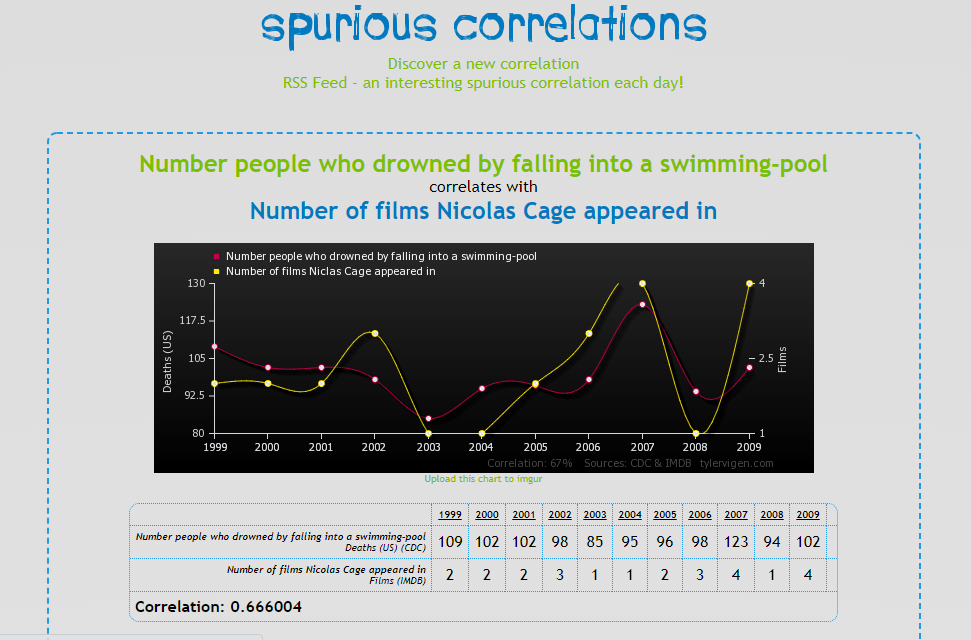
\includegraphics[width=0.8\linewidth]{imagenes/Spurious} 

}

\caption{Correlación espuria}\label{fig:unnamed-chunk-2}
\end{figure}

\textbf{Falacia de la anti-correlación}

No sé puede creer qué porque la correlación no es causalidad, las correlaciones no sirven para nada.

Por otra parte, W. Sosa señala que las siguientes aseveraciones son verdaderas. Puede haber:

\begin{enumerate}
\def\labelenumi{\arabic{enumi}.}
\tightlist
\item
  Correlación sin causalidad.
\item
  Causalidad sin correlación.
\item
  \textbf{La causalidad puede ir en una dirección y la correlación en la opuesta}.
\end{enumerate}

\hypertarget{quuxe9-es-eviews}{%
\section{¿Qué es Eviews?}\label{quuxe9-es-eviews}}

EViews es un \textbf{paquete econométrico, estadístico y de pronóstico moderno} que ofrece potentes herramientas analíticas dentro de una interfaz flexible y fácil de usar. Con EViews, se puede administrar datos de manera rápida y eficiente, realizar análisis econométricos y estadísticos, generar pronósticos o simulaciones de modelos y producir gráficos y tablas de alta calidad para su publicación o inclusión en otras aplicaciones.

La interfaz de usuario de EViews simplifica cada paso del proceso, desde la entrada e importación de datos, hasta la visualización de datos, análisis estadístico, estimación, pronóstico y resolución de modelos, salida de presentación de calidad de publicación.

\hypertarget{por-quuxe9-deberuxeda-utilizar-eviews}{%
\subsection{¿Por qué debería utilizar Eviews?}\label{por-quuxe9-deberuxeda-utilizar-eviews}}

Se tiene muchas opciones cuando se trata de software. Como ser:

\begin{itemize}
\tightlist
\item
  Excel
\item
  Stata
\item
  Minitab
\item
  RStudio
\item
  SAS
\item
  MatLab
\item
  OxMetrics
\end{itemize}

Entonces, ¿por qué debería elegir EViews?

\begin{itemize}
\item
  La innovadora interfaz EViews es fácil de usar, ya que ha sido diseñada desde cero para aprovechar los sistemas operativos modernos de Windows. La mayoría de los usuarios pueden dominar la interfaz a los pocos minutos de haber sido introducidos por primera vez a EViews. No hay una sintaxis complicada que aprender: ¡unos pocos golpes del mouse o clics del teclado y listo!
\item
  EViews se integra con sus otros productos de Windows. Además de abrir y guardar en una amplia gama de formatos de archivo diferentes (desde páginas web hasta Excel, Stata o SAS), EViews admite tecnologías estándar de Windows como copiar y pegar, vincular e incrustar objetos y conexiones ODBC.
\end{itemize}

Por otra parte, aunque el diseño principal de EViews presenta una interfaz de usuario con mouse, EViews también ofrece un extenso lenguaje de programación y comandos. Todas las acciones en EViews se pueden programar para automatizar tareas repetitivas o para mantener un registro de su trabajo.

\hypertarget{duxf3nde-puedo-obtener-muxe1s-informaciuxf3n}{%
\subsection{¿Dónde puedo obtener más información?}\label{duxf3nde-puedo-obtener-muxe1s-informaciuxf3n}}

Se puede tener mayor información en la página ofical de \href{http://www.eviews.com/}{Eviews}. Donde se puede obtener:

\begin{itemize}
\tightlist
\item
  Tutoriales en línea para explorar más funciones de EViews.
\item
  Una descripción más detallada de EViews.
\item
  Más información sobre lo que puede hacer EViews, consulte la lista de funciones de EViews.
\item
  Ejemplos y guías de algunas características nuevas agregadas en la última versión de EViews, EViews 11, vea nuestra página de ejemplos.
\end{itemize}

\hypertarget{conceptos-buxe1sicos-de-estaduxedstica-y-econometruxeda}{%
\chapter{Conceptos básicos de estadística y econometría}\label{conceptos-buxe1sicos-de-estaduxedstica-y-econometruxeda}}

\hypertarget{estaduxedstica}{%
\section{Estadística}\label{estaduxedstica}}

La estadística nos permitirá que a partir de un conjunto de datos realizar análisis, inferencia, estimar distribuciones de probabilidad, es decir, es un conjunto de métodos que estudian la recolección, análisis e interpretación de datos, ayudando en la toma de decisiones o para explicar condiciones regulares o irregulares de algún fenómeno o estudio aplicado, de ocurrencia en forma aleatoria o condicional \citep{Wooldridge2010}.

\hypertarget{conceptos-buxe1sicos}{%
\subsection{Conceptos básicos}\label{conceptos-buxe1sicos}}

\begin{itemize}
\item
  \textbf{Variables aleatorias:} una variable aleatoria X es una función cuyos valores son números reales y dependen de una distribución de probabilidad.
\item
  \textbf{Distribuciones de probabilidad:} una distribución de probabilidad describe el rango de valores que puede tomar una variable aleatoria y la probabilidad asignada a cada valor o rango de valores.
\item
  \textbf{Ley de los grandes números:} cuanto mayor sea el tamaño de la muestra, mayor será el ajuste entre la distribución teórica sobre la que se basa la muestra. La frecuencia relativa de los resultados de un cierto experimento aleatorio, tiende a estabilizarse en cierto número, que es precisamente la probabilidad, cuando el experimento se realiza muchas veces.
\item
  \textbf{Teorema del limite central:} la media muestral de un conjunto de n variables muestreadas en forma independiente a partir de una misma \emph{distribución f(x)} se ajusta a una distribución aproximada Normal. En otras palabras, la distribución del promedio de un conjunto de variables aleatorias depende tanto de la cantidad de variables aleatorias promediadas como de la incertidumbre aportada por cada variables.
\end{itemize}

\hypertarget{tipo-de-variables}{%
\subsubsection{Tipo de variables}\label{tipo-de-variables}}

\textbf{Variable} es una característica que al ser medida en diferentes individuos es susceptible de adoptar diferentes valores. Se tienen variables cualitativas (expresan características, cualidades) y cuantitativas (expresan cantidades numéricas).

Una variable aleatoria es una característica que toma diferentes valores, cada uno con una probabilidad previamente definida. Este valor es la realización de la variable.

Tipos de variables: cualitativas y cuantitativas

\hypertarget{momentos-estaduxedsticos}{%
\subsection{Momentos estadísticos}\label{momentos-estaduxedsticos}}

Las distribuciones de probabilidad, se describen mediante 3 tipos de parámetros, indicadores o ``estadísticos'', que son valores que muestran alguna de sus características:

\begin{itemize}
\tightlist
\item
  \textbf{Estadístico de Tendencia Central:} es un valor representativo de un conjunto de datos, \emph{el primer momento}, mide la tasa esperada de retornos sobre un proyecto en particular, los estadísticos comunes incluyen a la media (promedio), mediana (centro de la distribución) y moda (valor de ocurrencia mas frecuente).
\item
  \textbf{Estadístico de Dispersión:} \emph{El segundo momento}, dan una idea de qué tan aglomerado o disperso se pueden encontrar los valores alrededor del centro de la distribución.
\item
  \textbf{Estadístico de Forma:} Precisan otras características particulares de la distribución, como puede ser:

  \begin{itemize}
  \tightlist
  \item
    Su simetría ( \emph{tercer momento})
  \item
    La importancia relativa de los valores extremos ( \emph{cuarto momento})
  \end{itemize}
\end{itemize}

\hypertarget{tendencia-central}{%
\subsubsection{Tendencia central}\label{tendencia-central}}

La expresión corriente de promedio, suele en la mayoría de los casos referirse a la media aritmética.

Tendencia central: Media (promedio), mediana (centro de la distribución), moda (el valor que se presenta con mayor frecuencia).

Es la medida de posición o promedio más conocida, por su gran estabilidad es la preferida en el muestreo, sus fórmulas admiten tratamiento algebraico. Su desventaja principal, es ser muy sensible a cambios en sus valores u observaciones, también, cuando alguno de sus valores extremos es demasiado grande o pequeño (outliers).

Se define como la \textbf{suma de todos los valores observados, divididos por el número total de observaciones}

\[\bar{X} = \mu = \frac{\sum_{i=1}^n x_i}{n}\]
Propiedades de la media:

\begin{itemize}
\tightlist
\item
  La suma de las desviaciones respecto a la media, siempre serán iguales a cero.
\item
  La media aritmética de una variable por una constante, es igual a la constante por la media aritmética de la variable.
\item
  La media aritmética de una constante es igual a la constante.
\item
  La media aritmética de una variable más una constante, es igual a la media aritmética de la variable más la constante.
\item
  La media aritmética de la suma de dos variables, es igual a la suma de las dos medias correspondiente a las dos variables.
\item
  La media aritmética de dos muestras, es igual, a la media ponderada de las submuestras, siendo sus ponderaciones los tamaños de esas submuestras.
\end{itemize}

\hypertarget{dispersiuxf3n}{%
\subsubsection{Dispersión}\label{dispersiuxf3n}}

Mide la extensión de una distribución, la cual es una medida de riesgo. La extensión o amplitud de una distribución mide la variabilidad de una variable, es decir, el potencial de que una variable pueda caer en diferentes regiones de la distribución, en otras palabras, los potenciales escenarios de resultados.

Se puede estimar a partir de: varianza, desviación estándar, rango, coeficiente de variación, percentiles.

Las medidas de dispersión más conocidas y utilizadas son la varianza y la desviación típica o estándar. Esta última, es la raíz cuadrada de aquélla.

La varianza se define como: la media aritmética de los cuadrados de las diferencias (desviaciones) entre los valores que toma la variable y su media aritmética. Su símbolo es \(S^2\) en la muestra, \(\sigma^2\) (sigma al cuadrado) en la población.

Se utiliza el momento de orden 2 con respecto a la media.

\[S^2 = \frac{\sum_{i=1}^n (x_i - \bar{x})^2}{n}\]

\[\sigma^2 = \frac{\sum_{i=1}^n (X_i - \mu)^2}{N}\]

\textbf{Desviación típica o estándar:} indica en promedio como se dispersa una observación con respecto a la media aritmética. También es útil para describir cuanto se apartan las observaciones individuales con respecto a la media, se le conoce como resultado estándar.

\[S = \sqrt{S^2}\]
\[\sigma = \sqrt{\sigma^2}\]

En otras palabras:
- Es la distancia que tienen los datos con respecto a su media
- La desviación estándar es la raíz cuadrada de la varianza
- Para una distribución normal cerca del 68\% de la probabilidad está dentro de + o -- una desviación estándar de la media (95\% para 2 y 99\% para 3)

Regla empírica:
Distribución de probabilidad de variable aleatoria continua cuya forma es simétrica y acampanada y sus parámetros son una media y una desviación estándar.

\begin{itemize}
\tightlist
\item
  Alrededor del 68\% de las observaciones se encuentran en el intervalo 𝜇±𝜎.
\item
  Alrededor del 95\% de las observaciones se encuentran en el intervalo 𝜇±2𝜎.
\item
  Alrededor del 99\% de las observaciones se encuentran en el intervalo 𝜇±3𝜎.
\end{itemize}

\hypertarget{simetruxeda}{%
\subsubsection{Simetría}\label{simetruxeda}}

Coeficiente de asimetría:
\[m_3 = \frac{\sum_{i=1}^n (x_i - \bar{x})^3}{n}\]
1. \(A_s = 0\) la distribución es simétrica.
2. \(A_s >0\) la distribución es asimétrica positiva.
3. \(A_s <0\) la distribución es asimétrica negativa.

El alargamiento es la medida de la asimetría de una distribución. Mide la desviación de una distribución.

Una distribución normal no está alargada y tiene un alargamiento de 0. En distribuciones alargadas, la diferencia entre el resultado más probable y el promedio puede ser muy significativa.

Es importante conocer y estudiar las colas de la distribución ya que nos van a indicar valores extremos, por ejemplo, si seanaliza los rendimientos de una empresa, la cola izquierda indica pérdidas y la cola derecha ganancias.

\hypertarget{curtosis}{%
\subsubsection{Curtosis}\label{curtosis}}

La curtosis es una medida de altura de la curva y por tanto está representada por el \textbf{cuarto momento de la media.}

\[m_4 = \frac{\sum_{i=1}^n (x_i - \bar{x})^4}{n}\]
1. \(A_p = 3\) la distribución es normal o mesocúrtica.
2. \(A_p >3\) la curva es leptocúrtica o apuntado.
3. \(A_p <3\) la curva es platicúrtica o achatada.

La curtosis mide la forma de una distribución, en otras palabras, mide el punto más alto de una distribución.

Una distribución normal tiene una curtosis de 3 ó un exceso de curtosis de 0.

Distribuciones más picudas tienen valores de curtosis más altos, generalmente se calcula el exceso de curtosis haciendo referencia a la normal

\hypertarget{correlaciuxf3n}{%
\subsection{Correlación}\label{correlaciuxf3n}}

Un análisis de correlación permite diagnosticar el nivel o grado de asociación entre dos variables. Así pues, mediante el coeficiente de correlación de Pearson (\textbf{r}), se puede apreciar si las variables estan asociadas positivamente (\textbf{r \textgreater{} 0}); si se mueven en direcciones opuestas (\textbf{r \textless{} 0}); o si no están relacionadas o son independientes (\textbf{r = 0}).

Por otra parte, el coeficiente de correlación de Pearson se utiliza para relaciones líneas y no así para relaciones no lineales, donde se emplea el coeficiente de Spearman.

\[ r = \frac{\sum_{i=1}^{n}(x_i-\bar{x})(y_i-\bar{y})}{\sqrt{\sum_{i=1}^{n}(x_i-\bar{x})^2}\sqrt{\sum_{i=1}^{n}(y_i-\bar{y})^2}} \]

\hypertarget{econometruxeda}{%
\section{Econometría}\label{econometruxeda}}

\hypertarget{regresiuxf3n-lineal}{%
\subsection{Regresión lineal}\label{regresiuxf3n-lineal}}

El objetivo de la regresión lineal es \textbf{minimizar la distancia entre los puntos de un diagrama de dispersión (considerando que una linea no puede pasar perfectamente por todos los puntos)}. Ahora bien ¿Pueden ustedes encontrar la recta que minimice la distancia entre todos los puntos? Si son honestos seguro respondieron que no \citep{Maddala1996}.

\begin{figure}

{\centering 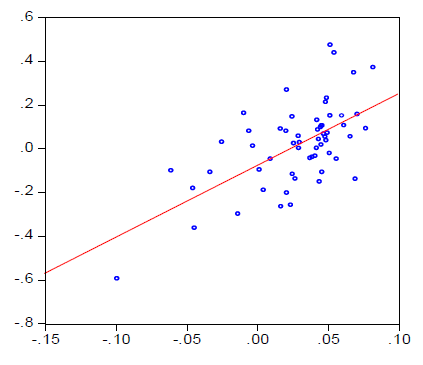
\includegraphics[width=0.8\linewidth]{imagenes/regresion} 

}

\caption{Regresión lineal}\label{fig:unnamed-chunk-3}
\end{figure}

\hypertarget{muxe9todo-de-muxednimo-cuadrados-ordinarios}{%
\subsubsection{Método de Mínimo Cuadrados Ordinarios}\label{muxe9todo-de-muxednimo-cuadrados-ordinarios}}

La Función de Regresión Lineal Poblacional:
\[Y_i = \beta_0 + \beta_1 X_i + \epsilon_i \]
La Función de Regresión Lineal Muestral:
\[\hat{Y}_i = \hat{\beta}_0 + \hat{\beta}_1 X_i + \hat{\epsilon}_i\]
Lo que se pretende es estimar los parámetros mediante el \{\bf método de mínimo cuadrados ordinarios\}, así pues, se minimiza en la muestra el error cuadrático medio (mean squared error):
\[\widehat{MSE}(\hat{\beta}_0, \hat{\beta}_1) \equiv \frac{1}{n}\sum_{i=1}^{n}{(Y_i - (\hat{\beta}_0 + \hat{\beta}_1 X_i))^2}\]
Depúes de minimizar el error cuadrático medio se obtiene:

\begin{enumerate}
\def\labelenumi{\arabic{enumi}.}
\tightlist
\item
  El intercepto:
  \[\hat{\beta}_0 = \bar{Y} – \hat{\beta}_1 \bar{X}\]
\item
  La pendiente:
  \[\hat{\beta}_1 = \frac{\sum(X_i – \bar{X}) (Y_i – \bar{Y})} {\sum(X_i – \bar{X})^2}\]
\end{enumerate}

\hypertarget{ejemplo-de-un-modelo-de-regresiuxf3n}{%
\subsubsection{Ejemplo de un modelo de regresión}\label{ejemplo-de-un-modelo-de-regresiuxf3n}}

\textbf{¿Cuál es la relación entre el salario y el nivel de eduación de las personas?}

Se puede considerar que a mayor nivel de educación mayor salario, así también, otras variables.

Modelo de regresión:
\(\mathrm{Salario}_{t}=\alpha+\beta_{1}\mathrm{Niv.eduación}_{t}+\beta_{2}\mathrm{Exp.laboral}_{t}+\beta_{3} \mathrm{Edad}_{t}+\beta_{4}\mathrm{Género}_{t}+\beta_{5}\mathrm{Skill}_{t}+\epsilon_{t}\)

Se presentan las siguientes preguntas:

\begin{enumerate}
\def\labelenumi{\arabic{enumi}.}
\tightlist
\item
  ¿Cómo interpretamos \(\beta_{1}\)?
\item
  Un año de educación adicional se correlaciona con un \(\beta_{1}\) aumento de unidades en el salario de un individuo (controlando por todas las otras variables).
\item
  ¿Los términos \(\beta_{i}\) son parámetros de población o estadísticas de muestra?
\item
  Las letras griegas denotan \textbf{parámetros de población} y suus estimaciones obtienen sombreros, por ejemplo, \(\hat{\beta}_i\).
\item
  ¿Podemos interpretar las estimaciones para \(\beta_{1}\) como causal?
\item
  ¿Qué es \(\epsilon_{t}\)?
\item
  ¿Qué supuestos imponemos al realizar estimaciones con MCO?
\end{enumerate}

\begin{itemize}
\tightlist
\item
  \textbf{Supuestos:}

  \begin{itemize}
  \tightlist
  \item
    La relación entre el salario y las variables explicativas es lineal en parámetros, y \(\epsilon_{t}\) afecta de manera aditiva.
  \item
    Las variables explicativas son \textbf{exógenas}, es decir, \(E[\epsilon_{t}|X] = 0\).
  \item
    Por lo general, también ha asumido algo como: \(E[\epsilon_{t}] = 0\), \(E[\epsilon_t^2] = \sigma^2\), \(Cov[\epsilon_t \epsilon_j] = 0\) for \(t \neq j\).
  \item
    Se distribuye normalmente \(\epsilon_t\).
  \end{itemize}
\end{itemize}

\textbf{¿Qué tan importantes pueden ser la regresión por mínimos cuadrados ordinarios (MCO)?}

Es una herramienta poderosa y flexible. Sin embargo, los resultados que se pueden estimar requirieron suposiciones.

\textbf{La vida real a menudo viola estos supuestos.}

Entonces, la pregunta es: \textbf{¿qué sucede cuando violamos estos supuestos?}

\begin{itemize}
\tightlist
\item
  ¿Podemos encontrar una solución? (Especialmente: cómo/cuándo es \(\beta\) \emph{causal}?)
\item
  ¿Qué sucede si no aplicamos (o no podemos) una solución?
\end{itemize}

MCO todavía hace algunas cosas asombrosas, pero necesita saber cuándo ser \textbf{cauteloso, confiado o dudoso}.

\hypertarget{instrucciones-de-uso-de-eviews}{%
\chapter{Instrucciones de uso de EViews}\label{instrucciones-de-uso-de-eviews}}

\hypertarget{cargar-los-datos}{%
\section{Cargar los datos}\label{cargar-los-datos}}

\hypertarget{crear-un-archivo-de-trabajo}{%
\subsection{Crear un archivo de trabajo}\label{crear-un-archivo-de-trabajo}}

\begin{enumerate}
\def\labelenumi{\arabic{enumi}.}
\tightlist
\item
  Abre el programa EViews y ve a \textbf{File\textgreater New\textgreater Workfile}.
\item
  Para datos de sección cruzada selecciona \textbf{Unstructured/Undated} e introduce el tamaño de la muestra en el campo \textbf{End observation}.
\item
  Para datos temporales selecciona la frecuencia e introduce en el campo \textbf{Start observation} la fecha inicial y en \textbf{End observation} la fecha final.
\item
  Confirma \textbf{OK} y guarda el archivo de trabajo en \textbf{File\textgreater Save as}.
\end{enumerate}

\begin{figure}

{\centering 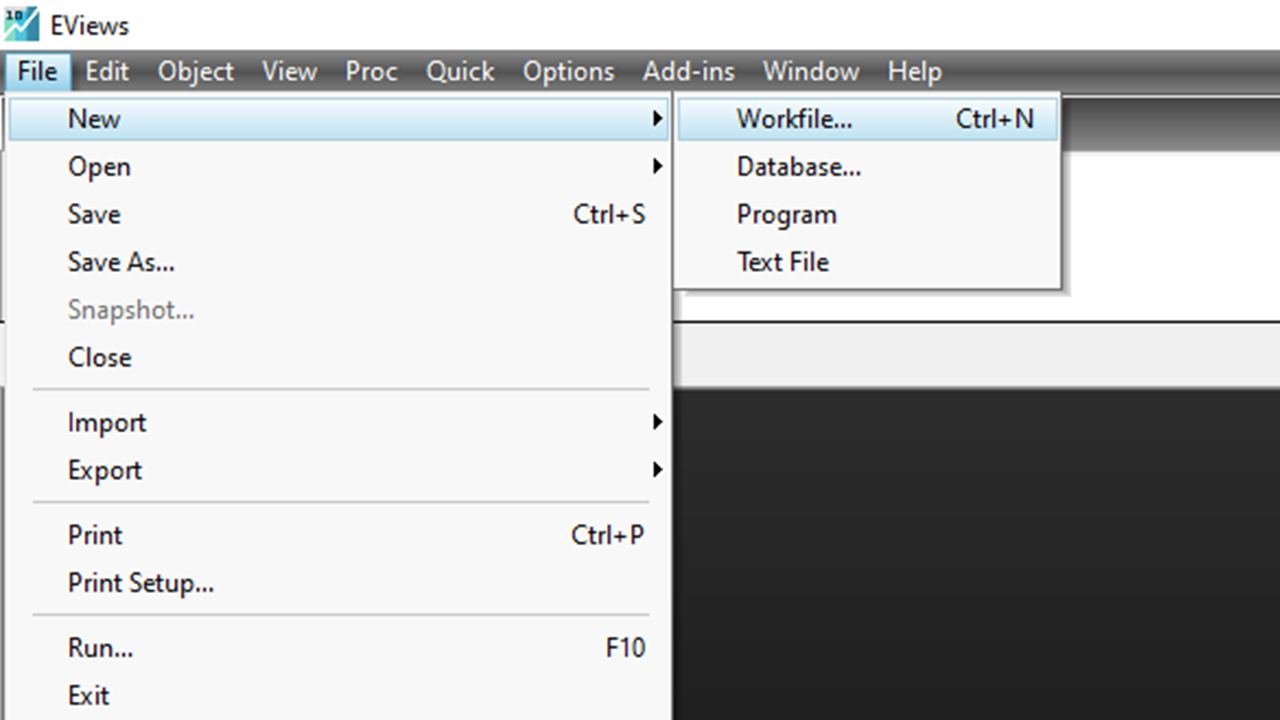
\includegraphics[width=0.75\linewidth]{imagenes/3_1} 

}

\caption{Crear un archivo de trabajo}\label{fig:unnamed-chunk-4}
\end{figure}

\hypertarget{abrir-un-archivo-de-trabajo-ya-existente}{%
\subsection{Abrir un archivo de trabajo ya existente}\label{abrir-un-archivo-de-trabajo-ya-existente}}

\begin{enumerate}
\def\labelenumi{\arabic{enumi}.}
\tightlist
\item
  En \textbf{File\textgreater Open\textgreater Workfile} puedes buscar un archivo de trabajo en el disco.
\item
  Los archivos de trabajo de EViews tienen extensión \textbf{wf1}.
\end{enumerate}

\hypertarget{introducir-datos-a-mano}{%
\subsection{Introducir datos a mano}\label{introducir-datos-a-mano}}

\begin{enumerate}
\def\labelenumi{\arabic{enumi}.}
\tightlist
\item
  Crea un archivo de trabajo (ya se realizo en el 3.1.1) y selecciona \textbf{Quick\textgreater Empty Group (Edit Series)}.
\item
  Sube con el cursor una vez para que se pueda ver la primera fila.
\item
  En \textbf{la primera fila introduce el nombre de la variable} y en la columna debajo los valores.
\item
  Cierra la ventana y a la pregunta \textbf{Delete Untitled GROUP?} contesta \textbf{Yes}.
\item
  En \textbf{File\textgreater Save As} puedes guardar el archivo de trabajo con extensión por defecto wf1.
\end{enumerate}

\hypertarget{importar-datos-de-una-hoja-de-cuxe1lculo}{%
\subsection{Importar datos de una hoja de cálculo}\label{importar-datos-de-una-hoja-de-cuxe1lculo}}

\begin{enumerate}
\def\labelenumi{\arabic{enumi}.}
\tightlist
\item
  Los datos deben estar en una hoja de Excel en columnas con el nombre de las variables en la primera fila.
\item
  Selecciona \textbf{File\textgreater Import\textgreater Import from file\ldots{}}
\item
  Busca en el disco duro tu hoja de cálculo, selecciona y confirma \textbf{Abrir}.
\end{enumerate}

\begin{figure}

{\centering 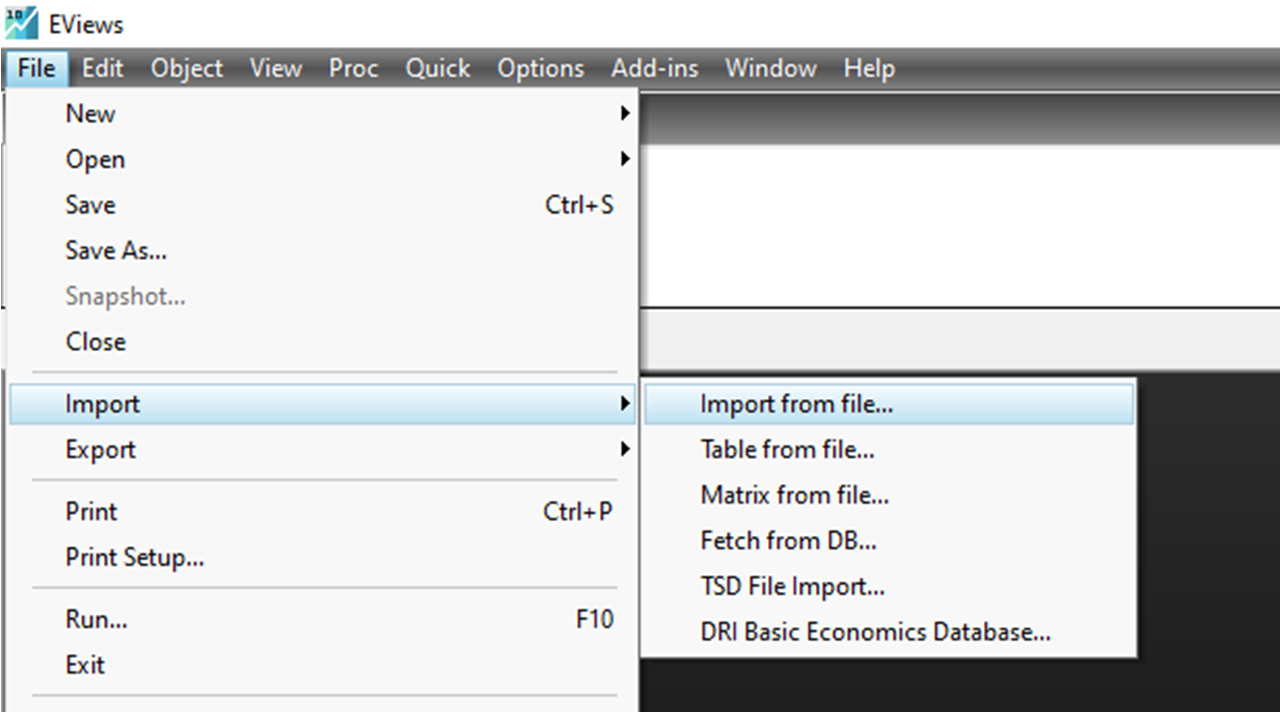
\includegraphics[width=0.75\linewidth]{imagenes/3_2} 

}

\caption{Importar datos de una hoja de cálculo}\label{fig:unnamed-chunk-5}
\end{figure}

\hypertarget{transformaciuxf3n-y-creaciuxf3n-de-variables}{%
\section{Transformación y creación de variables}\label{transformaciuxf3n-y-creaciuxf3n-de-variables}}

\hypertarget{seleccionar-objetos-en-un-grupo-de-trabajo}{%
\subsection{Seleccionar objetos en un grupo de trabajo}\label{seleccionar-objetos-en-un-grupo-de-trabajo}}

\begin{enumerate}
\def\labelenumi{\arabic{enumi}.}
\tightlist
\item
  En la ventana del archivo de trabajo puedes seleccionar objetos (variables, tablas, gráficos) con el cursor.
\item
  Mantén presionada la tecla \textbf{Ctrl}.
\item
  Con el cursor haz click para seleccionar y deseleccionar objetos.
\item
  Libera la tecla \textbf{Ctrl} y los objetos permanecerán seleccionados.
\end{enumerate}

\hypertarget{borrar-una-variable}{%
\subsection{Borrar una variable}\label{borrar-una-variable}}

\begin{enumerate}
\def\labelenumi{\arabic{enumi}.}
\tightlist
\item
  En el archivo de trabajo selecciona la variable que desees borrar.
\item
  Haz click con el botón derecho del ratón en la variable.
\item
  Selecciona la opción \textbf{Delete}. ¡Atención, variables borradas son irrecuperables!
\end{enumerate}

\hypertarget{renombrar-una-variable}{%
\subsection{Renombrar una variable}\label{renombrar-una-variable}}

\begin{enumerate}
\def\labelenumi{\arabic{enumi}.}
\tightlist
\item
  En el archivo de trabajo selecciona la variable que desees renombrar.
\item
  En el archivo de trabajo haz click con el botón derecho del ratón en la variable.
\item
  Selecciona la opción \textbf{Rename\ldots{}}
\item
  En \textbf{Name to identify object} introduce el nuevo nombre y confirma OK.
\end{enumerate}

\hypertarget{editar-una-variable}{%
\subsection{Editar una variable}\label{editar-una-variable}}

\begin{enumerate}
\def\labelenumi{\arabic{enumi}.}
\tightlist
\item
  En el archivo de trabajo haz doble click en la variable.
\item
  Haz click en el bot´on \textbf{Edit +/--} y cambia los valores moviéndote con el cursor.
\item
  Cierra la ventana y a la pregunta \textbf{Delete Untitled GROUP?} contesta \textbf{Yes}.
\end{enumerate}

\hypertarget{editar-varias-variables-a-la-vez}{%
\subsection{Editar varias variables a la vez}\label{editar-varias-variables-a-la-vez}}

\begin{enumerate}
\def\labelenumi{\arabic{enumi}.}
\tightlist
\item
  Selecciona las variables que desees editar (3.2.1).
\item
  Haz click con el botón derecho del ratón y selecciona \textbf{Open\textgreater as Group}.
\item
  Haz click en el botón \textbf{Edit +/--} y cambia los valores moviéndote con el cursor.
\item
  Cierra la ventana y a la pregunta \textbf{Delete Untitled GROUP?} contesta \textbf{Yes}.
\end{enumerate}

\hypertarget{crear-una-variable-a-partir-de-variables-existentes.-retardos.}{%
\subsection{Crear una variable a partir de variables existentes. Retardos.}\label{crear-una-variable-a-partir-de-variables-existentes.-retardos.}}

\begin{enumerate}
\def\labelenumi{\arabic{enumi}.}
\tightlist
\item
  Abre tu fichero de trabajo y ve al menú \textbf{Quick\textgreater Generate series\ldots{}}
\item
  Introduce la fórmula en el campo \textbf{Enter equation} y confirma \textbf{OK}.
\item
  Nota: Una expresión como \textbf{lprecio=log(precio)} crea una nueva variable \textbf{lprecio} que contiene el logaritmo de las observaciones de precio. Otras expresiones comunes son la suma \textbf{x=y+z}, la diferencia \textbf{x=y-z}, el producto **y=x*z\textbf{, el cociente }y=x/z\textbf{, la potencia }y=xˆ2\textbf{, el logaritmo }y=log(x)\textbf{, la exponencial }y=exp(z)\textbf{, el operador lógico }y=(x\textless=0)\textbf{ o funciones estadísticas }\href{mailto:dx=x-@mean}{\nolinkurl{dx=x-@mean}}(x)**.
\item
  Nota: Si \textbf{x} es una variable, \textbf{x(-k)} es el retardo \textbf{k-}ésimo de la variable.
\item
  Nota: En \textbf{Help\textgreater Function Reference} hay una lista de operadores y funciones.
\end{enumerate}

\hypertarget{copiar-una-o-varias-variables-u-objetos-de-un-archivo-de-trabajo-a-otro}{%
\subsection{Copiar una o varias variables (u objetos) de un archivo de trabajo a otro}\label{copiar-una-o-varias-variables-u-objetos-de-un-archivo-de-trabajo-a-otro}}

\begin{enumerate}
\def\labelenumi{\arabic{enumi}.}
\tightlist
\item
  Abre en el programa los dos archivos de trabajo.
\item
  En la ventana del grupo de origen, señala o selecciona las variables a copiar.
\item
  Selecciona \textbf{Edit\textgreater Copy} o presiona \textbf{Ctrl-C}.
\item
  Activa la ventana del grupo de destino haciendo click en ella y selecciona \textbf{Edit\textgreater Paste} o presiona \textbf{Ctrl-V}.
\item
  Nota: Si el tamaño de la muestra no es igual, el programa recorta o amplia el tamaño de la serie: si lo recorta sólo se conservan las primeras observaciones; si lo amplia, rellena los huecos con no disponible (\textbf{NA}).
\end{enumerate}

\hypertarget{crear-un-objeto-escalar-o-nuxfamero}{%
\subsection{Crear un objeto escalar o número}\label{crear-un-objeto-escalar-o-nuxfamero}}

\begin{enumerate}
\def\labelenumi{\arabic{enumi}.}
\tightlist
\item
  Ve a la línea de comando, el espacio en blanco justo debajo de la opción \textbf{File}.
\item
  Escribe la ecuación precedida de la opción \textbf{scalar}, por ejemplo, la instrucción \textbf{scalar \href{mailto:preciomedio=@mean}{\nolinkurl{preciomedio=@mean}}(precio)}.
\item
  Presiona la tecla \textbf{Enter}.
\item
  Nota: Los objetos escalares no se pueden abrir en ventanas: haz doble click en el escalar para ver su valor en la esquina inferior izquierda de la ventana de EViews.
\end{enumerate}

\hypertarget{vista-de-objetos}{%
\subsection{Vista de objetos}\label{vista-de-objetos}}

Los objetos que se pueden encontrar en EViews son los siguientes:

\begin{figure}

{\centering 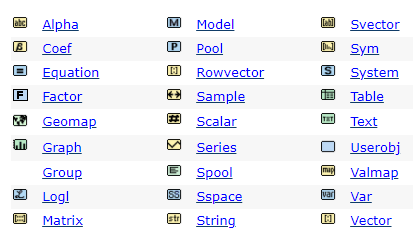
\includegraphics[width=0.75\linewidth]{imagenes/3_3} 

}

\caption{Objetos en Eviews}\label{fig:unnamed-chunk-6}
\end{figure}

\hypertarget{estaduxedsticos-descriptivos}{%
\section{Estadísticos descriptivos}\label{estaduxedsticos-descriptivos}}

\hypertarget{estaduxedsticos-de-una-o-muxe1s-variables}{%
\subsection{Estadísticos de una o más variables}\label{estaduxedsticos-de-una-o-muxe1s-variables}}

\begin{enumerate}
\def\labelenumi{\arabic{enumi}.}
\tightlist
\item
  Marca las variables (3.2.1) cuyos estadísticos desees calcular.
\item
  En \textbf{Quick\textgreater Group Statistics} selecciona \textbf{Descriptive Statistics\textgreater Common sample} para obtener estadísticos relativos a cada variable individual como la media, mediana, etc., de cada una de las variables.
\item
  En \textbf{Quick\textgreater Group Statistics} selecciona:
\end{enumerate}

\begin{enumerate}
\def\labelenumi{(\alph{enumi})}
\tightlist
\item
  \textbf{Covariances} para la matriz de varianzas y covarianzas.
\item
  \textbf{Correlations} para la matriz de correlaciones.
\end{enumerate}

\begin{enumerate}
\def\labelenumi{\arabic{enumi}.}
\setcounter{enumi}{3}
\tightlist
\item
  Nota: Se puede guardar los resultados congelando la ventana.
\end{enumerate}

\hypertarget{congelar-una-tabla-o-gruxe1fico-para-guardar}{%
\subsection{Congelar una tabla o gráfico para guardar}\label{congelar-una-tabla-o-gruxe1fico-para-guardar}}

\begin{enumerate}
\def\labelenumi{\arabic{enumi}.}
\tightlist
\item
  Cuando tengas un resultado, una tabla o un gráfico, presiona el botón \textbf{Freeze}.
\item
  En la nueva ventana que se abre presiona el botón \textbf{Name}, elige un nombre y confirma \textbf{OK}.
\end{enumerate}

\hypertarget{gruxe1ficos-de-una-variable}{%
\subsection{Gráficos de una variable}\label{gruxe1ficos-de-una-variable}}

\begin{enumerate}
\def\labelenumi{\arabic{enumi}.}
\tightlist
\item
  En \textbf{Quick\textgreater Series Statistics} selecciona:
\end{enumerate}

\begin{enumerate}
\def\labelenumi{(\alph{enumi})}
\tightlist
\item
  \textbf{Histogram and stats} para el histograma y los estadísticos básicos.
\item
  \textbf{Correlogram} para obtener un correlograma de la serie en niveles (Level), primeras (\textbf{1st difference}) y segundas diferencias (\textbf{2nd difference}).
\end{enumerate}

\begin{enumerate}
\def\labelenumi{\arabic{enumi}.}
\setcounter{enumi}{1}
\tightlist
\item
  También puedes hacer doble click en la variable y en \textbf{View} seleccionar la opción correspondiente; vuelve a los datos con \textbf{View \textgreater{} SpreadSheet}.
\item
  Para guardar los resultados congela la ventana.
\end{enumerate}

\hypertarget{gruxe1ficos-de-dos-variables}{%
\subsection{Gráficos de dos variables}\label{gruxe1ficos-de-dos-variables}}

\begin{enumerate}
\def\labelenumi{\arabic{enumi}.}
\tightlist
\item
  En \textbf{Quick\textgreater Graph\ldots{}} introduce las variables (la primera variable aparecerá en el eje horizontal) y confirma \textbf{OK}.
\item
  Selecciona el tipo de gráfico, como el de puntos \textbf{Scatter}.
\item
  Si lo deseas, presiona el botón \textbf{Options} para realizar cambios en la visualización.
\item
  Confirma \textbf{OK} para ver el gráfico. Para guardarlo haz click en el botón \textbf{Name}.
\item
  Nota: Haciendo doble click en el gráfico abres de nuevo la pantalla de opciones.
\end{enumerate}

\hypertarget{estimaciuxf3n-y-contrastes}{%
\section{Estimación y contrastes}\label{estimaciuxf3n-y-contrastes}}

\hypertarget{estimar-por-muxednimos-cuadrados-ordinarios-mco}{%
\subsection{Estimar por mínimos cuadrados ordinarios (MCO)}\label{estimar-por-muxednimos-cuadrados-ordinarios-mco}}

\begin{enumerate}
\def\labelenumi{\arabic{enumi}.}
\tightlist
\item
  En \textbf{Quick\textgreater Estimate equation} escribe la ecuaci´on de manera abreviada, por ejemplo \textbf{log(y) c x}, donde la \textbf{c} indica la ordenada en el origen.
\item
  Confirma \textbf{OK} para ver la ventana con los resultados. Usa el botón \textbf{Name} para guardar la regresión activa. Para guardar definitivamente los resultados puedes congelar la ventana.
\item
  Nota: En el botón \textbf{View} puedes acceder a opciones y contrastes.
\item
  Nota: En \textbf{c(k)} se guarda el valor de la estimación del coeficiente \textbf{k} y lo puedes usar para generar nuevas variables como \textbf{ygorro=c(1)+c(2)\emph{x\textbf{ o escalares como }scalar media=c(1)+c(2)}@mean(x)}.
\item
  Nota: En \textbf{resid} se guardan los residuos de la regresión hasta que corras otra regresión. Si quieres guardarlos puedes generar una nueva variable que contenga los residuos, como \textbf{residuos2=resid}.
\end{enumerate}

\hypertarget{contraste-de-restricciones-lineales}{%
\subsection{Contraste de restricciones lineales}\label{contraste-de-restricciones-lineales}}

\begin{enumerate}
\def\labelenumi{\arabic{enumi}.}
\tightlist
\item
  En la ventana de la regresión correspondiente ve a \textbf{View\textgreater Coefficient Tests} y elige la opción \textbf{Wald-Coefficient Restrictions\ldots{}}
\item
  En el campo \textbf{Coefficient restrictions separated by commas} introduce la restricción \textbf{c(1)=c(2)} o restricciones \textbf{c(1)=2c(2)},\textbf{c(3)=0}* y confirma \textbf{OK}.
\item
  Para guardar los resultados congela la ventana.
\item
  Para volver a la regresión selecciona \textbf{View\textgreater Estimation Output}.
\end{enumerate}

\hypertarget{contraste-de-heterocedasticidad-de-white}{%
\subsection{Contraste de heterocedasticidad de White}\label{contraste-de-heterocedasticidad-de-white}}

\begin{enumerate}
\def\labelenumi{\arabic{enumi}.}
\tightlist
\item
  En la ventana de la regresión correspondiente ve a \textbf{View\textgreater Residual Tests} y elige la opción \textbf{White Heteroskedasticity (cross-terms)}.
\item
  Para guardar los resultados congela la ventana.
\item
  Para volver a la regresión selecciona \textbf{View\textgreater Estimation Output}.
\end{enumerate}

\hypertarget{contraste-de-autocorrelaciuxf3n-de-breusch-godfrey}{%
\subsection{Contraste de autocorrelación de Breusch-Godfrey}\label{contraste-de-autocorrelaciuxf3n-de-breusch-godfrey}}

\begin{enumerate}
\def\labelenumi{\arabic{enumi}.}
\tightlist
\item
  En la ventana de la regresión correspondiente ve a \textbf{View\textgreater Residual Tests} y elige la opción \textbf{Serial Correlation LM Test}.
\item
  En el campo \textbf{Lags to include} especifica el número de retardos de los residuos que deseas considerar y confirma \textbf{OK}.
\item
  Para guardar los resultados congela la ventana. Para volver a los resultados de la regresión selecciona \textbf{View\textgreater Estimation Output}.
\end{enumerate}

\hypertarget{aplicaciones-empuxedricas}{%
\chapter{Aplicaciones empíricas}\label{aplicaciones-empuxedricas}}

\begin{quote}
``Con respecto al gobierno, los datos comparativos entre países indican que el consumo del gobierno está inversamente relacionado con el crecimiento, mientras que la inversión pública tiene poca relación con el crecimiento. Las tasas de crecimiento promedio están relacionadas positivamente con la estabilidad política, que puede aprovechar los beneficios de los derechos de propiedad seguros.''

--- Robert J. Barro
\end{quote}

\hypertarget{crecimiento-econuxf3mico}{%
\section{Crecimiento Económico}\label{crecimiento-econuxf3mico}}

El crecimiento económico es uno de los temas más estudiados y discutidos dentro de los estudios de macroeconomía aplicada, es así que dentro de la academia es importante examinar los factores que tienen efectos sobre el crecimiento económico. Así pues, \textbf{Chirwa y Odhiambo (2016)} señalan la distinción sobre los factores determinantes macroeconómicos del crecimiento económico en los países en desarrollo y desarrollados. Su estudio revela que en los países en desarrollo los determinantes macroeconómicos del crecimiento económico son: la ayuda externa, la inversión extranjera directa, la política fiscal, la inversión, el comercio, el desarrollo del capital humano, la demografía, la política monetaria, los recursos naturales, las reformas y los factores geográficos, regionales, políticos y financieros. Asimismo, en los países desarrollados son: capital físico, política fiscal, capital humano, comercio, demografía, política monetaria y factores financieros y tecnológicos.

Por otra parte, en el contexto de América Latina existe una discusión sobre los efectos de las exportaciones y de la demanda interna sobre el crecimiento económico. De esta manera, \textbf{Alvarado, Ochoa-Jiménez, y García-Tinisaray (2018)} mediante el marco teórico del modelo de crecimiento desarrollado por Bulmer-Thomas estiman un modelo econométrico de panel para los 28 países latinoamericanos. Sus resultados señalan que el efecto de la demanda interna en el crecimiento económico es mayor que el de las exportaciones. Asimismo, los resultados difieren cuando se clasifica por su nivel de ingreso per cápita. En los países de ingresos altos, las exportaciones desempeñan un papel más importante que la demanda interna para aumentar la producción, mientras que en los países de ingresos medianos-altos predomina el efecto de la demanda interna, y para los países de ingresos medianos-bajos no es concluyente.

¿Cuáles son los factores que afectan al crecimiento económico en Bolivia?

\begin{figure}

{\centering 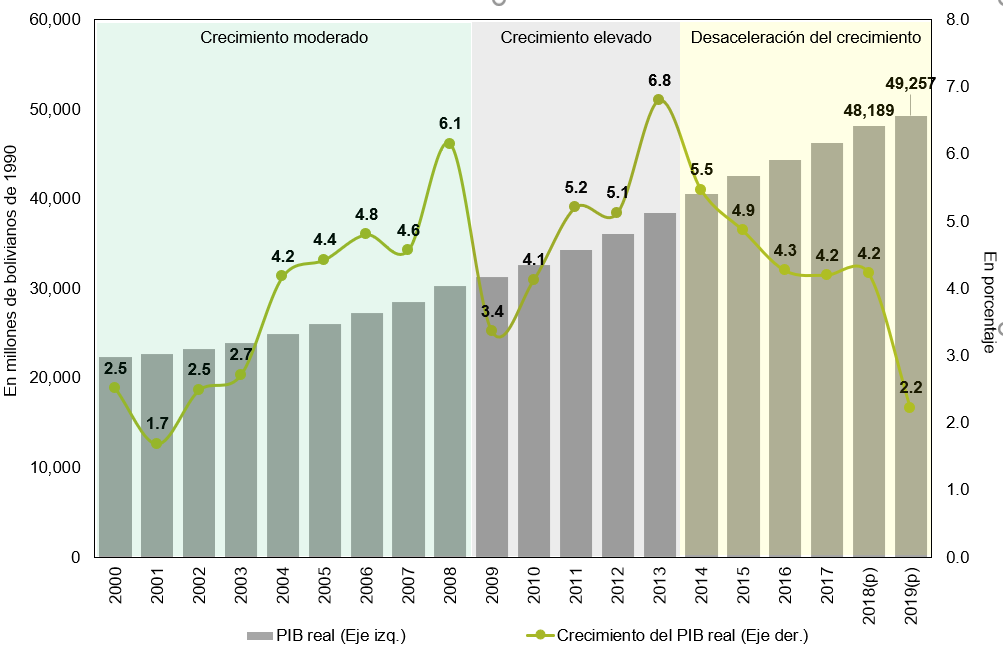
\includegraphics[width=0.8\linewidth]{imagenes/growth} 

}

\caption{Tasa de crecimiento económico}\label{fig:unnamed-chunk-7}
\end{figure}

\hypertarget{pronuxf3sticos}{%
\chapter{Pronósticos}\label{pronuxf3sticos}}

\begin{quote}
``Los resultados han sido prácticamente unánimes: la combinación de múltiples pronósticos conduce a una mayor precisión del pronóstico. En muchos casos, se pueden realizar mejoras drásticas en el rendimiento simplemente promediando los pronósticos.''

--- Robert Clemen
\end{quote}

\hypertarget{series-de-tiempo}{%
\section{Series de tiempo}\label{series-de-tiempo}}

Es un conjunto de observaciones sobre los valores de una variable en diferentes momentos, ordenada en periodos regulares (días, semanas, meses, etc.).

\begin{figure}

{\centering 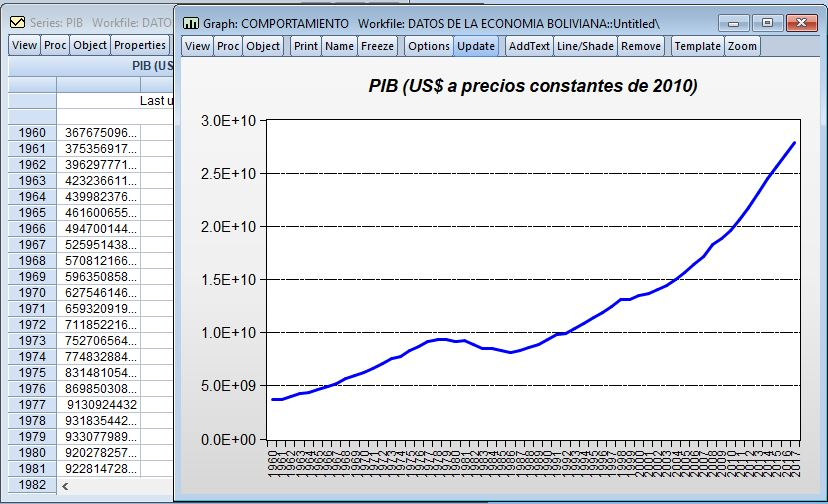
\includegraphics[width=0.8\linewidth]{imagenes/PIB} 

}

\caption{Producto Interno Bruto de Bolivia}\label{fig:unnamed-chunk-8}
\end{figure}

\hypertarget{modelos-arima}{%
\section{Modelos ARIMA}\label{modelos-arima}}

La publicación ``Times Series Análisis: Forecasting and Control'' de George Box y Gwilym en 1976 generó un nuevo conjunto de herramientas de predicción, cuyo procedimiento se llamó metodología Box- Jenkins; también técnicamente conocida como metodología ARIMA.

Los modelos ARIMA proporcionan otro enfoque para el pronóstico de series de tiempo, se basan en describir las autocorrelaciones y media móviles en los datos, razón por la que algunas veces se les denomina modelos ateóricos, donde no existe relación causal alguna a diferencia de los modelos clásicos de regresión.

La especificación del modelo se puede escribir de la siguiente manera:

\[ y_i = c + \rho_1 y_{t-1}+\dots + \sum_{i=1}^{p}\rho_p y_{t-p}+ \varepsilon_t - \theta_1 \varepsilon_{t-1}+\dots- \sum_{i=1}^{q}\theta_q \varepsilon _{t-q}\]

Dónde \(y_i\) es la serie diferenciada. Los ``predictores'' del lado derecho incluyen ambos valores rezagados de \(y_{t-1}\) y errores retrasados.

El objetivo de la metodología Box--Jenkins es identificar y estimar un modelo estadístico que puede ser interpretado como generador de la información de la muestra. En este sentido, si el modelo estimado es usado para la predicción debe suponerse que las características de la serie son constantes en el tiempo, especialmente para los periodos futuros. Por lo tanto, la predicción se efectúa sobre una base válida considerando que el modelo es estacionario o estable.

Las etapas que se deben seguir en la elaboración de un modelo ARIMA con fines predictivos son las siguientes:

\begin{enumerate}
\def\labelenumi{\arabic{enumi}.}
\tightlist
\item
  Identificación
\item
  Estiamción
\item
  Verificación
\item
  Pronóstico
\end{enumerate}

  \bibliography{book.bib,packages.bib}

\end{document}
